% Chapter added after v1.3.0: Conway maps, ratchets, problems M1 and M4, the tail criterion, Fourier decay.
\providecommand{\rhomin}{\rho_{\min}}
\providecommand{\fl}[1]{\lfloor #1\rfloor}
\providecommand{\ce}[1]{\lceil #1\rceil}
\providecommand{\Cm}{\mathrm{Col}_{\min}}
\chapter{Ratchets, Records and Tails}\label{rrt:chap:ratchets}

\noindent
This chapter collects work done after the first edition on five questions. What happens to the methods of this book on Conway's generalized Collatz maps? Is there an entropy argument behind the density results, and a ratchet argument of the kind that drives Parrondo's paradox? What becomes of Problems M1 and M4 of \cref{chap:missed}? How fast must the tail of the orbit minimum decay for Problem B1 to go through? And how fast do the Fourier coefficients of the Syracuse random variable really decay, which is Problem B2? Nothing here proves the conjecture. The chapter sharpens what a proof must do, and it finds the same constant in four places.

The results, in order.
\begin{enumerate}
\item \emph{Conway's maps} (Sections \ref{rrt:sec:conway} and \ref{rrt:sec:methods}). On the subclass with multipliers coprime to the modulus, the digit bijection, the Lyapunov function $n^{\theta}$, the martingale bound and the density one descent theorem all hold with full proofs (Theorems \ref{rrt:thm:bijection}, \ref{rrt:thm:lyap}, \ref{rrt:thm:density}). No method covers the whole class (Proposition \ref{rrt:prop:unprovable}).
\item \emph{Entropy} (Section \ref{rrt:sec:entropy}). The equipartition argument is the dual of the Lyapunov argument and gives the same exponent, $0.05004$ bits per step for the Collatz map (Theorem \ref{rrt:thm:duality}).
\item \emph{Ratchets} (Section \ref{rrt:sec:ratchet}). Two Conway maps with all orbits bounded can alternate to a map with all orbits divergent (Theorem \ref{rrt:thm:parrondo}). Measure preservation forbids this for a common modulus (Theorem \ref{rrt:thm:noparrondo}), and with two moduli the Collatz map itself is one of two losing games that win together (Theorem \ref{rrt:thm:resonance}).
\item \emph{Cycles} (Sections \ref{rrt:sec:exact} to \ref{rrt:sec:m4}). The sharp minimum inequality is an equality for the Christoffel cycle at every rung (Theorem \ref{rrt:thm:exact}). Problem M1 is false as stated and true in its exact form (Proposition \ref{rrt:prop:false}, Theorem \ref{rrt:thm:records}). For Problem M4 we give exact counts, a rigorous upper bound at every rung and a supermultiplicative lower bound (Table \ref{rrt:tab:rho}).
\item \emph{Tails} (Section \ref{rrt:sec:tail}). Granting Lau's theorem, the conjecture is equivalent to a polynomial bound on the tail of the orbit minimum, where Tao's theorem gives a logarithmic one (Theorem \ref{rrt:thm:tail}).
\item \emph{Fourier decay} (Section \ref{rrt:sec:fourier}). A single Fourier coefficient of the Syracuse variable at level $n$ can be computed in $O(n^2)$ operations (Proposition \ref{rrt:prop:fk}). We reproduce the exact table of \cref{chap:backward} to level $18$ and continue to level $2000$. The largest coefficient over powers of two appears to decay geometrically, like $n^{-3/2}\,3^{-0.05004\,n}$, and not like $n^{-2}$ (Table \ref{rrt:tab:fk}, Conjecture \ref{rrt:conj:fourier}).
\item \emph{Basins} (Section \ref{rrt:sec:basin}). In a $3x+d$ map with $312\,455$ cycles of one type, basin sizes are heavy tailed and one cycle captures $3.7$ percent of all starting values.
\end{enumerate}

The constant that keeps returning is the entropy deficit $\eta=1-h(\log 2/\log 3)=0.05004$. It is the Chernoff rate of the stopping time, the Sanov rate of the words that do not contract, the growth deficit of the words of a cycle, and, numerically, the rate at which the worst Fourier coefficient decays as a power of the modulus. Section \ref{rrt:sec:smm} says what the Switching MM viewpoint contributes to this picture.

Every theorem below is proved in full or marked as conditional or conjectural. None of the proofs has been refereed, and the attribution in Remark \ref{rrt:rem:hh} needs to be checked against the literature.


\section{Conway's generalization}\label{rrt:sec:conway}

\begin{definition}
A \emph{Conway map} with modulus $d\ge 2$ is a function $g:\Z\to\Z$ of the form
\[
g(n) = a_i n + b_i \qquad \text{for } n\equiv i \pmod d,\quad i=0,1,\dots,d-1,
\]
where the $a_i,b_i$ are rational numbers chosen so that $g(n)$ is always an integer.
\end{definition}

The Collatz map $T(n)=n/2$ for $n$ even, $T(n)=(3n+1)/2$ for $n$ odd, is the case $d=2$. Conway \cite{conway1972} proved that the purely multiplicative case $b_i=0$ already computes everything.

\begin{theorem}[Conway 1972]\label{rrt:thm:conway}
For every partial recursive function $f$ there is a Conway map $g(n)=a_i n$ such that, for every $n$, the orbit of $2^n$ under $g$ meets another power of two if and only if $f(n)$ is defined, and the first such power is then $2^{f(n)}$. Consequently no algorithm decides, given $g$ and $n$, whether the orbit of $n$ under $g$ ever reaches $1$.
\end{theorem}

Conway later turned the construction into the programming language FRACTRAN \cite{conway1987}, published, fittingly for this chapter, in a volume edited by the information theorist Thomas Cover. Kurtz and Simon \cite{kurtz2007} sharpened Theorem \ref{rrt:thm:conway}: the set of Conway maps for which every orbit reaches $1$ is $\Pi^0_2$ complete. Both facts are recalled in \cref{chap:intro} and used in \cref{chap:quantifier}.

Conway's own favourite example \cite{conway2013} is the \emph{amusical permutation}
\[
\gamma(2k)=3k,\qquad \gamma(4k+1)=3k+1,\qquad \gamma(4k-1)=3k-1 .
\]
It is a bijection of the positive integers. Its known cycles are $\{1\}$, $\{2,3\}$, $\{4,6,9,7,5\}$ and a cycle of length twelve through $44$. Whether the orbit of $8$ is infinite is open. The drift heuristic gives a growth factor $(3/2)^{1/2}(3/4)^{1/2}=(9/8)^{1/2}$ per step, and after $2000$ steps the orbit of $8$ has indeed reached about $10^{43}$.

\subsection{The coprime class}
Between the Collatz map and the full Conway class sits the family studied by Matthews and Watts \cite{matthews1984,matthews1985}.

\begin{definition}\label{rrt:def:mw}
A \emph{coprime Conway map} with modulus $d$ and multipliers $m_0,\dots,m_{d-1}$ is
\[
T(x)=\frac{m_i x - r_i}{d}\qquad\text{for } x\equiv i \pmod d ,
\]
where the $m_i$ are positive integers with $\gcd(m_i,d)=1$ and the $r_i$ are integers with $r_i\equiv i\,m_i \pmod d$. The \emph{digit} of $x$ is $x_0(x)=x \bmod d$, and the digit sequence is $x_j = x_0(T^j x)$. The \emph{multiplier} after $k$ steps is
\[
M_k(x)=\prod_{j=0}^{k-1}\frac{m_{x_j}}{d}.
\]
\end{definition}

The Collatz map has $d=2$, $(m_0,m_1)=(1,3)$ and $r_1=-1$. The first result is the general form of the parity vector theorem of Terras \cite{terras1976} and Everett \cite{everett1977}.

\begin{theorem}[Digit bijection]\label{rrt:thm:bijection}
Let $T$ be a coprime Conway map. For every $k\ge 1$ the map
\[
x \bmod d^k \;\longmapsto\; (x_0,x_1,\dots,x_{k-1})
\]
is a well defined bijection from $\Z/d^k\Z$ onto $\{0,\dots,d-1\}^k$. Hence if $x$ is uniform on a complete residue system modulo $d^k$, its first $k$ digits are independent and uniform on $\{0,\dots,d-1\}$.
\end{theorem}

\begin{proof}
By induction on $k$, on any set of integers with common digits $x_0,\dots,x_{k-2}$ the iterate $T^{k-1}$ is a single affine map, so that
\[
T^{k-1}(x)-T^{k-1}(x') = \frac{m_{x_0}\cdots m_{x_{k-2}}}{d^{\,k-1}}\,(x-x') .
\]
Assume the statement for $k-1$. If $x\equiv x' \pmod{d^k}$ then the first $k-1$ digits agree and the right side is divisible by $d$, so the $k$th digits agree: the map is well defined. Conversely, if the first $k$ digits agree, then $x\equiv x'\pmod{d^{k-1}}$ by induction and the left side is divisible by $d$. Since the product of the $m$'s is coprime to $d$, we get $x\equiv x' \pmod{d^k}$: the map is injective. Both sets have $d^k$ elements.
\end{proof}

Equivalently, $T$ extends to the $d$ adic integers $\Z_d$, preserves Haar measure, and is conjugate to the one sided Bernoulli shift on $d$ symbols with the uniform product measure. Coprimality is essential. For a general Conway map the digits form at best a Markov chain with a nonuniform stationary law \cite{leigh1986}, and Section \ref{rrt:sec:ratchet} shows how much can go wrong.

\section{Do our methods apply?}\label{rrt:sec:methods}

The optimization view of this book replaces the two branch map by a one parameter family of Lyapunov functions $V_\theta(n)=n^\theta$ and then optimizes over $\theta$. For a coprime Conway map define the \emph{drift} and the \emph{moment function}
\[
\mu=\frac1d\sum_{i=0}^{d-1}\log\frac{m_i}{d},\qquad
\rho(\theta)=\frac1d\sum_{i=0}^{d-1}\Big(\frac{m_i}{d}\Big)^{\theta},\qquad
\Lambda(\theta)=\log\rho(\theta).
\]

\begin{theorem}[Lyapunov and martingale structure]\label{rrt:thm:lyap}
Let $T$ be a coprime Conway map and let $x$ be Haar distributed on $\Z_d$, or uniform modulo $d^k$.
\begin{enumerate}
\item[(a)] $\E\,[M_k^\theta]=\rho(\theta)^k$ for every real $\theta$, and $M_k^\theta/\rho(\theta)^k$ is a martingale in $k$.
\item[(b)] $\Lambda$ is convex with $\Lambda(0)=0$ and $\Lambda'(0)=\mu$. There is $\theta>0$ with $\rho(\theta)<1$ if and only if $\mu<0$, that is, if and only if $\prod_i m_i<d^{\,d}$.
\item[(c)] If $\mu<0$ and some $m_i>d$, there is a unique $\theta^*>0$ with $\rho(\theta^*)=1$, the process $M_k^{\theta^*}$ is a martingale, and
\[
\Prob\Big(\sup_{k\ge 0} M_k \ge u\Big)\le u^{-\theta^*}\qquad (u\ge 1).
\]
\item[(d)] For every $k$, $\;\Prob(M_k\ge 1)\le \rhomin^{\,k}$, where $\rhomin=\min_{\theta\ge 0}\rho(\theta)$.
\end{enumerate}
\end{theorem}

\begin{proof}
Part (a) is Theorem \ref{rrt:thm:bijection}: the factors of $M_k$ are independent and each has $\theta$th moment $\rho(\theta)$. Part (b) is convexity of a cumulant generating function. In (c), $\rho(\theta)\to\infty$ as $\theta\to\infty$ because some $m_i/d>1$, and convexity gives uniqueness; the bound is Doob's maximal inequality for the positive martingale $M_k^{\theta^*}$. Part (d) is Markov's inequality applied to $M_k^{\theta}$, optimized over $\theta$.
\end{proof}

Parts (c) and (d) are the two halves of the programme. Part (c) is the martingale duality: the Lundberg exponent $\theta^*$ is the tail index of the largest excursion of an orbit. Part (d) is the optimization step: choosing $\theta$ to minimize $\rho$ is a one dimensional convex programme, the Chernoff bound, and it plays the role that the majorization step plays for the Collatz map in \cref{chap:momentum,chap:mmcollatz}.

For Collatz, $\rho(\theta)=\tfrac12\big(2^{-\theta}+(3/2)^{\theta}\big)$, so $\rho(1)=1$ and $\theta^*=1$ exactly. The idealized orbit $n M_k$ is itself a martingale, and the largest excursion has the Pareto tail $1/u$, in agreement with the stochastic models of Lagarias and Weiss \cite{lagarias1992}. The minimizer solves $3^{\theta}=\log 2/\log(3/2)$, so
\[
\theta_{\min}=0.4881,\qquad \rhomin=0.96591 ,
\]
which are the Chernoff exponent and factor of \cref{chap:stochastic} and Appendix A. Figure \ref{rrt:fig:lambda} shows $\Lambda$.

\begin{figure}[t]
\centering
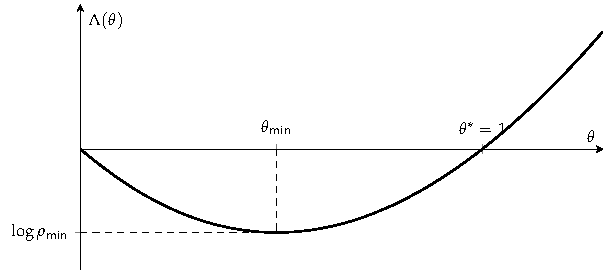
\includegraphics[width=0.78\textwidth]{figures/ch20r_lambda.pdf}
\caption{The cumulant function $\Lambda(\theta)=\log\tfrac12(2^{-\theta}+(3/2)^{\theta})$ of the Collatz map. Its minimum gives the stopping time exponent, its positive root the excursion tail.}
\label{rrt:fig:lambda}
\end{figure}

Table \ref{rrt:tab:maps} lists the constants for several coprime maps. Since $\rho(1)=\sum_i m_i/d^2$, we have $\theta^*=1$ exactly when $\sum_i m_i=d^2$. The Collatz map belongs to this \emph{martingale family}, and so does the modulus four map with multipliers $(1,3,5,7)$.

\begin{table}[t]
\centering
\small
\begin{tabular}{llrrrr}
\toprule
$d$ & $(m_i)$ & $\mu$ & $\theta_{\min}$ & $\eta$ (bits) & $\theta^*$\\
\midrule
2 & $(1,3)$ & $-0.1438$ & $0.488$ & $0.0500$ & $1$\\
2 & $(1,5)$ & $+0.1116$ & $0$ & $0$ & none\\
3 & $(1,2,4)$ & $-0.4055$ & $1.476$ & $0.3983$ & $3.499$\\
3 & $(1,2,7)$ & $-0.2189$ & $0.329$ & $0.0523$ & $0.662$\\
4 & $(1,3,5,7)$ & $-0.2228$ & $0.469$ & $0.0717$ & $1$\\
\bottomrule
\end{tabular}
\caption{Drift $\mu$, optimal Lyapunov exponent $\theta_{\min}$, equipartition exponent $\eta=-\log_2\rhomin$ and Lundberg exponent $\theta^*$ for coprime Conway maps.}
\label{rrt:tab:maps}
\end{table}

\subsection{From multipliers to integers}
Iterating Definition \ref{rrt:def:mw} gives $T^k(x)=M_k(x)\,x+R_k(x)$ with $|R_k|\le c\,k\,K^k$, where $c=\max_i|r_i|/d$ and $K=\max(1,\max_i m_i/d)$. This is enough to transfer Theorem \ref{rrt:thm:lyap}(d) to the integers.

\begin{theorem}[Density one descent]\label{rrt:thm:density}
Let $T$ be a coprime Conway map with $\mu<0$. For each $k$, the set of positive integers $n$ with $|T^j(n)|<n$ for some $j\le k$ has lower density at least $1-\rhomin^{\,k}$. In particular almost every positive integer, in the sense of natural density, has an iterate smaller than itself.
\end{theorem}

\begin{proof}
Fix $k$. The multiplier $M_k$ depends only on $n \bmod d^k$ and takes finitely many values, so there is $\lambda_k<1$ with $M_k\le\lambda_k$ whenever $M_k<1$. By Theorems \ref{rrt:thm:bijection} and \ref{rrt:thm:lyap}(d) the residue classes with $M_k<1$ have proportion at least $1-\rhomin^{\,k}$. For $n$ in such a class, $|T^k(n)|\le \lambda_k n+c\,k\,K^k<n$ as soon as $n>c\,k\,K^k/(1-\lambda_k)$.
\end{proof}

For Collatz this is the theorem of Terras and Everett with the sharp rate $0.96591^k=2^{-0.05004\,k}$ found by Lagarias \cite{lagarias1985}. The proof used nothing about $3x+1$ beyond coprimality, so the answer to the first question is yes: on the coprime class the methods of this book transfer line by line.

\subsection{Where the methods must stop}
The methods cannot extend to every Conway map, for a reason that does not depend on the method.

\begin{proposition}\label{rrt:prop:unprovable}
Let $\mathcal{T}$ be any sound, recursively axiomatized theory, for example ZFC if it is sound. There is a Conway map $g$ all of whose orbits reach $1$ such that $\mathcal{T}$ does not prove this. In particular $g$ admits no Lyapunov function whose descent property is provable in $\mathcal{T}$.
\end{proposition}

\begin{proof}
The set of Conway maps for which $\mathcal{T}$ proves that every orbit reaches $1$ is recursively enumerable, and by soundness it is contained in the set of maps for which this is true. If the two sets were equal, a $\Pi^0_2$ complete set \cite{kurtz2007} would be $\Sigma^0_1$, which is false.
\end{proof}

So a uniform certificate is impossible, and any proof technique must use special structure. For the coprime class that structure is Theorem \ref{rrt:thm:bijection}. Conway's universal maps are multiplicative with multipliers sharing factors with $d$; they lie outside the coprime class, their digits are not equidistributed, and the cumulant function $\Lambda$ no longer describes them. Whether undecidability can occur \emph{inside} the coprime class is, as far as we know, open (Problem \ref{rrt:op:undecidable}).

\section{Entropy and equipartition}\label{rrt:sec:entropy}

The asymptotic equipartition property \cite{cover2006} says that for an independent source with entropy $H$ per symbol, strings of length $k$ split into a typical set of about $e^{kH}$ strings carrying almost all the probability, and an atypical remainder. For a coprime Conway map the source is the digit sequence, which by Theorem \ref{rrt:thm:bijection} is uniform with entropy $H=\log d$: the Collatz map produces exactly one fair bit per step. Since all strings are equally likely, the content of equipartition lies in the \emph{types}. Write $q$ for the empirical distribution of the first $k$ digits. Then
\[
\frac1k\log M_k=\sum_i q_i\log\frac{m_i}{d},
\]
so descent is a statement about the type alone. Typical strings have $q$ close to uniform and multiplier close to $e^{k\mu}$. Orbits that fail to descend must have a type in the half space $\{q:\sum_i q_i\log(m_i/d)\ge 0\}$.

\begin{theorem}[Entropy and Lyapunov duality]\label{rrt:thm:duality}
Let $T$ be a coprime Conway map with $\mu<0$ and let $u$ be the uniform law on digits. Then
\[
\eta\;:=\;\min\Big\{D(q\,\|\,u)\;:\;\sum_i q_i\log\frac{m_i}{d}\ge 0\Big\}\;=\;-\log_2\rhomin ,
\]
where $D$ is relative entropy in bits. The number of digit strings of length $k$ with $M_k\ge 1$ is $2^{k(\log_2 d-\eta)+o(k)}$.
\end{theorem}

\begin{proof}
The count is Sanov's theorem, or the method of types \cite{cover2006}: a type class has $2^{k(\log_2 d-D(q\|u))+o(k)}$ elements and there are polynomially many types. The identity is Cram\'er's theorem, which is the Lagrangian dual of the constrained minimization: the minimizing $q$ is the exponential tilt $q_i\propto (m_i/d)^{\theta_{\min}}$, and $\theta_{\min}$ is the multiplier of the constraint.
\end{proof}

The left side is an entropy and the right side is a Lyapunov function. The optimal exponent $\theta_{\min}$ of the optimization approach is the Lagrange multiplier of the equipartition constraint, and the supermartingale $n^{\theta_{\min}}$ is the exponentially tilted measure in disguise. For the Collatz map the constraint reads $q_1\ge\theta_c$ with $\theta_c=\log 2/\log 3=0.6309$, and
\[
\eta = 1-h(\theta_c)= 0.05004 \text{ bits} = -\log_2 0.96591 ,
\]
where $h$ is the binary entropy function. Of the $2^k$ parity strings of length $k$, about $2^{0.94996\,k}$ fail to contract.

\subsection{What equipartition cannot do}
So there is an equipartition argument, and it is sharp. It has three limits, and stating them precisely is the main lesson of this section.

First, equipartition bounds the size of the atypical set and says nothing about whether it is empty. The Collatz conjecture is the statement that one specific countable set, the positive integers inside $\Z_2$, avoids the atypical set of divergent and cyclic parity sequences. That set has Haar measure zero, so no statement that holds almost everywhere can see it. This is the integrality principle of \cref{chap:synthesis}.

Second, there is an entropy budget. An integer $n$ supplies $\log_2 n$ bits. The idealized walk needs $\log n/|\mu|$ steps to descend from $n$ to $1$, and each step consumes one fair bit, so the descent consumes
\[
\frac{\log 2}{|\mu|}\,\log_2 n \;=\; 4.82\,\log_2 n \text{ bits.}
\]
The orbit must therefore look random for a stretch almost five times longer than its seed. Theorem \ref{rrt:thm:bijection} certifies only the first $\log_2 n$ digits. Beyond that point the conjecture is a pseudorandomness statement about the map $x\mapsto 3x+1$ acting on binary digits, and equipartition, which is a statement about true randomness, is silent. This is the gap that Tao \cite{tao2022} narrows by showing that the relevant distribution stabilizes modulo powers of three, which yields descent to almost bounded values for almost all $n$ in logarithmic density.

Third, the map is two to one on $\Z_2$ and so erases one bit per step, the choice of preimage. Entropy production at rate $\log 2$ is what makes the forward dynamics a contraction on average, and it is the same fact that makes the backward tree of \cref{chap:backward} grow.

\section{Ratchets and Parrondo's paradox}\label{rrt:sec:ratchet}

A Brownian ratchet \cite{ajdari1992} is a particle in an asymmetric sawtooth potential that is switched on and off. With the potential on, the particle is trapped. With it off, the particle diffuses symmetrically. Alternating the two produces a net current, although neither regime does. Parrondo's games \cite{harmer1999} are the discrete version; \cref{sec:ch5:parrondo} used them as an analogy for momentum, and here the games are arithmetic. Game $A$ is a coin with win probability $\tfrac12-\epsilon$. Game $B$ uses a coin with win probability $\tfrac1{10}-\epsilon$ when the capital is a multiple of three and $\tfrac34-\epsilon$ otherwise. Both lose, and alternations of them win.

The structural point is that game $B$ is a random Conway map: the rule depends on the capital modulo $d$. The paradox rests on one fact. A naive analysis of game $B$ at $\epsilon=0$ assumes the capital is uniform modulo three and finds the win probability $\tfrac13\cdot\tfrac1{10}+\tfrac23\cdot\tfrac34=0.533$. The true stationary law of the capital modulo three is $(5,2,6)/13$, which puts more weight on the bad residue and gives exactly $\tfrac12$. Mixing in game $A$ pushes the residues back toward uniform and releases the favourable drift.

That is precisely the status of the Collatz heuristic. The drift $\mu=\tfrac12\log\tfrac34$ is the naive calculation, which assumes uniform residues. The following example shows that for Conway maps the naive calculation can fail completely, and deterministically.

\begin{theorem}[A deterministic Parrondo pair]\label{rrt:thm:parrondo}
Define two Conway maps with modulus four on the nonnegative integers by
\[
A(n)=\begin{cases}3n+1 & n \text{ even}\\ \lfloor n/4\rfloor & n \text{ odd,}\end{cases}
\qquad
B(n)=\begin{cases}3n+1 & n \text{ odd}\\ \lfloor n/4\rfloor & n \text{ even.}\end{cases}
\]
\begin{enumerate}
\item[(a)] Every orbit of $A$ enters the cycle $\{0,1\}$.
\item[(b)] Every orbit of $B$ enters the fixed point $\{0\}$ or the cycle $\{1,4\}$.
\item[(c)] Every orbit of the alternation $C=B\circ A$ tends to infinity, and $C(n)=9n+4$ for all even $n$.
\end{enumerate}
\end{theorem}

\begin{proof}
(a) If $n\ge 1$ is odd, $A(n)=\lfloor n/4\rfloor<n$. If $n\ge 2$ is even, $3n+1$ is odd and $A^2(n)=\lfloor(3n+1)/4\rfloor<n$. So every orbit descends until it reaches $\{0,1\}$, and $A(0)=1$, $A(1)=0$.

(b) If $n\ge 2$ is even, $B(n)=\lfloor n/4\rfloor<n$, and $B(0)=0$. If $n$ is odd, $3n+1$ is even and $B^2(n)=\lfloor(3n+1)/4\rfloor\le n$ with equality only at $n=1$, where $B(1)=4$ and $B(4)=1$.

(c) If $n$ is even then $A(n)=3n+1$ is odd, so $C(n)=3(3n+1)+1=9n+4$, which is again even. The even numbers are invariant and $C^k(n)\ge 9^k n+4$ there. If $n$ is odd then $C(n)\le\lfloor n/4\rfloor<n$ unless $\lfloor n/4 \rfloor$ is odd, in which case $C(n)$ is even. A strictly decreasing sequence of odd positive integers is finite, so the orbit reaches an even number.
\end{proof}

Table \ref{rrt:tab:parrondo} shows the three orbits of $27$.

\begin{table}[t]
\centering
\small
\begin{tabular}{ll}
\toprule
map & orbit of $27$\\
\midrule
$A$ & $27,\,6,\,19,\,4,\,13,\,3,\,0,\,1,\,0,\,1,\dots$\\
$B$ & $27,\,82,\,20,\,5,\,16,\,4,\,1,\,4,\,1,\dots$\\
$B\circ A$ & $27,\,1,\,0,\,4,\,40,\,364,\,3280,\,29524,\,265720,\dots$\\
\bottomrule
\end{tabular}
\caption{Two bounded games and their unbounded alternation.}
\label{rrt:tab:parrondo}
\end{table}

The mechanism is a ratchet with no noise at all. Each map uses its expanding branch to push the state into the residue class on which its own contracting branch acts, so each map alone is trapped. Alternation moves the state, at each step, into the class on which the \emph{next} map expands, and the pawl never engages.

Now compare with Collatz. Each of $A$ and $B$ multiplies by $3$ on half of the residues and by $1/4$ on the other half, so the naive drift of each is $\tfrac12\log 3+\tfrac12\log\tfrac14=\tfrac12\log\tfrac34$, which is \emph{exactly the Collatz drift} $\mu$. The naive drift of $C$ is $2\mu<0$, and the truth is $+\log 9$. The stationary parity law of $A$ as a Markov chain on the parity bit is $(\tfrac13,\tfrac23)$ on (even, odd), with drift $\tfrac13\log 3-\tfrac23\log 4=-0.558$, although every orbit of $A$ itself ends in $\{0,1\}$. The naive number is wrong for all three maps, in both directions.

\subsection{Why Collatz is not a ratchet}
What separates Collatz from this example is Theorem \ref{rrt:thm:bijection}.

\begin{theorem}[No ratchet under measure preservation]\label{rrt:thm:noparrondo}
Let $T_A$ and $T_B$ be coprime Conway maps with the same modulus $d$ and drifts $\mu_A,\mu_B$. Under Haar measure on $\Z_d$, the expected logarithmic multiplier of any composition of $p$ copies of $T_A$ and $q$ copies of $T_B$, in any order, equals $p\,\mu_A+q\,\mu_B$. In particular two maps with negative drift cannot be combined into one with positive drift.
\end{theorem}

\begin{proof}
Each map preserves Haar measure, so at every stage of the composition the current point is Haar distributed and its digit is uniform. The expected logarithmic multiplier of that stage is therefore the drift of the map applied, and expectations add without any independence assumption.
\end{proof}

So in the coprime class the naive drift is the true drift, in the Haar sense, and there is nothing for a ratchet to rectify. Parrondo effects belong to the part of Conway's class in which the residue chain has a nonuniform stationary law, and the correct drift there is $\sum_i\pi_i\log a_i$ with $\pi$ that stationary law, as in the Markov analysis of Leigh \cite{leigh1986}. Theorem \ref{rrt:thm:noparrondo} is again a statement about Haar almost every point. The conjecture asserts that the integers do not conspire to behave like the orbits of Theorem \ref{rrt:thm:parrondo}(c), locked onto the expanding branch.

\subsection{Resonance: a Parrondo pair that contains the Collatz map}\label{rrt:sec:resonance}
Theorem \ref{rrt:thm:noparrondo} needs a common modulus. With two moduli the ratchet returns, and the Collatz map itself can be one of the two games. The reason is a resonance: the multiplier $3$ of the Collatz map is the modulus of the second game. Since $(3x+1)/2\equiv 2 \pmod 3$ for every odd $x$, the odd branch of the Collatz map deposits every point in the class $2$ modulo $3$. The Collatz map preserves Haar measure on $\Z_2$ and does not preserve it on $\Z_3$.

For $m\in\{7,13,19,25\}$, so that $m\equiv 1 \pmod 6$ and $m<27$, let $B_m$ be the coprime Conway map with modulus three and multipliers $(1,1,m)$,
\[
B_m(x)=\frac{x}{3},\quad \frac{x-1}{3},\quad \frac{m x-2}{3}\qquad\text{for } x\equiv 0,1,2 \pmod 3 .
\]

\begin{theorem}[Collatz as game $A$]\label{rrt:thm:resonance}
Let $T$ be the Collatz map, let $B=B_m$ as above and let $C=B\circ T$.
\begin{enumerate}
\item[(a)] Both games lose: $\mu_T=\tfrac12\log\tfrac34<0$ and $\mu_B=\tfrac13\log\tfrac{m}{27}<0$, and by Theorem \ref{rrt:thm:density} almost every positive integer has a smaller iterate under $T$ and under $B$.
\item[(b)] Haar measure on $\Z_2\times\Z_3$ is invariant under $C$. Under it the multipliers of successive rounds are independent and identically distributed, equal to
\[
\frac{m}{2}\ \text{ w.p. } \tfrac12,\qquad \frac16\ \text{ w.p. } \tfrac13,\qquad \frac{m}{6}\ \text{ w.p. } \tfrac16 .
\]
\item[(c)] The drift of a round is
\[
\mu_C=\mu_T+\tfrac12\log\frac{m}{3}+\tfrac12\mu_B=\frac16\log\frac{m^4}{1728},
\]
which is positive for every $m\ge 7$. The naive value $\mu_T+\mu_B$ is negative.
\item[(d)] The first $k$ rounds of $n$ depend only on $n \bmod 6^k$, and the set of positive integers $n$ with $|C^j(n)|>n$ for some $j\le k$ has lower density at least $1-\rho_C^{\,k}$, where $\rho_C=\min_{\theta\ge 0}\E\,[M^{-\theta}]<1$ and $M$ is the round multiplier of (b). In particular almost every positive integer has a larger iterate under $C$.
\end{enumerate}
\end{theorem}

\begin{proof}
(a) is a computation. For (b), let $(x,y)$ be Haar distributed on $\Z_2\times\Z_3$; the integers sit on the diagonal. The parity $d$ of $x$ is a fair bit, and by Theorem \ref{rrt:thm:bijection} $T(x)$ is Haar on $\Z_2$ and independent of $d$; all of this is independent of $y$. If $d=0$ the $3$ adic coordinate moves to $y'=y/2$, which is again Haar because division by two is an isometry of $\Z_3$. The digit $i$ of $y'$ is then uniform on $\{0,1,2\}$, and $B(y')$ is Haar and independent of $i$, again by Theorem \ref{rrt:thm:bijection}. If $d=1$ the $3$ adic coordinate moves to $(3y+1)/2$, which lies in the class $2$, so $i=2$, and the round acts on $y$ by
\[
y\longmapsto \frac{m\,(3y+1)/2-2}{3}=\frac{m\,y+(m-4)/3}{2},
\]
an isometry of $\Z_3$ since $m\equiv 1 \pmod 3$ and $m$ is a unit. In both cases $B$ acts on the $2$ adic coordinate by $x'\mapsto(m_i x'-r_i)/3$, an isometry of $\Z_2$ because $m_i$ is odd. So after one round the point is again Haar distributed and independent of the symbol $(d,i)$, whose law is $(1,2)$ with probability $\tfrac12$ and $(0,i)$ with probability $\tfrac16$ each. Induction gives the independence of successive rounds, and the multipliers are $\tfrac32\cdot\tfrac m3$, $\tfrac12\cdot\tfrac13$, $\tfrac12\cdot\tfrac13$ and $\tfrac12\cdot\tfrac m3$.

(c) is the mean of the logarithm of the multiplier in (b). For (d), a round reads one binary digit and at most one ternary digit, and a round that reads no ternary digit acts on the $3$ adic coordinate by the isometry $y\mapsto(my+(m-4)/3)/2$ of (b), while every branch of $B$ is an isometry of $\Z_2$, so $k$ rounds depend only on $n\bmod 6^k$ and on each class $C^k(n)=M_k n+R_k$ with $|R_k|\le c\,k\,K^k$. Since $\mu_C>0$ the function $\theta\mapsto\E[M^{-\theta}]$ has negative derivative at zero, so $\rho_C<1$, and Markov's inequality gives $\Prob(M_k\le 1)\le\rho_C^{\,k}$. On the remaining classes $M_k\ge\lambda_k>1$ and $|C^k(n)|>n$ for all large $n$, as in Theorem \ref{rrt:thm:density}.
\end{proof}

\begin{table}[t]
\centering
\small
\begin{tabular}{rrrrrr}
\toprule
$m$ & $\mu_B$ & $\mu_C$ & $\rho_C$ & $\theta^*_C$ & escaped\\
\midrule
7 & $-0.4500$ & $+0.0548$ & $0.9992$ & $0.058$ & $25.5\%$\\
13 & $-0.2436$ & $+0.4675$ & $0.9619$ & $0.328$ & $93.3\%$\\
19 & $-0.1171$ & $+0.7205$ & $0.9280$ & $0.414$ & $96.4\%$\\
25 & $-0.0257$ & $+0.9035$ & $0.9030$ & $0.457$ & $98.5\%$\\
\bottomrule
\end{tabular}
\caption{The pair (Collatz, $B_m$). Here $\theta^*_C$ solves $\E[M^{-\theta}]=1$, and the last column is the proportion of $n\le 20000$ whose orbit under $C=B_m\circ T$ exceeds $10^{80}$; the others enter a cycle. For $m=7$ the $40$ orbits still unresolved when the run stopped are counted as escaped.}
\label{rrt:tab:resonance}
\end{table}

Table \ref{rrt:tab:resonance} gives the constants. The law in (b) was checked exactly on all $1296$ residues modulo $6^4$ for $m=7$, and a simulation from random $4000$ bit integers gave a drift of $0.0559$ against the predicted $0.0548$. For $m=7$ every orbit of $B_m$ from $n\le 20000$ enters the fixed point $0$; for $m=13$ and $m=19$ every such orbit enters $0$ or a cycle ($13\,773$ and $3\,022$ of them a nontrivial one).

Three remarks. First, this answers the question left open after Theorem \ref{rrt:thm:noparrondo}: a Parrondo pair exists inside the coprime class as soon as the moduli differ, and the Collatz map is one of its members. Second, the case $m=7$ is striking because $B_7$ is strongly contracting, with $\prod m_i=7$ against $27$, and the pair still wins. Third, the theorem is a statement about density and not about every integer. An orbit of $C$ is a walk with positive drift that is captured if it ever wanders down to a cycle, and the walk heuristic puts the probability of capture from $n$ near $n^{-\theta^*_C}$. For $m=7$ that exponent is $0.058$, which is why three quarters of the integers below $20000$ are still captured; the theorem says the proportion tends to zero in the sense of (d), very slowly.

The same proof shows when the ratchet is absent: if every multiplier of each map is coprime to both moduli, then every branch is an isometry of the other coordinate, both maps preserve Haar measure on $\Z_{d_A}\times\Z_{d_B}$ (on $\Z_{\operatorname{lcm}(d_A,d_B)}$ if the moduli are not coprime), and Theorem \ref{rrt:thm:noparrondo} holds unchanged. A ratchet between coprime Conway maps therefore requires a resonance, a multiplier of one map sharing a prime with the modulus of the other. For the Collatz map the only resonant prime is three. This is the same $3$ adic nonuniformity that Tao \cite{tao2022} controls through the Syracuse random variable, seen here from the side of the ratchet.


\subsection{The Brownian picture}
There remains a real Brownian argument for Collatz, at the level of the idealized walk. By Theorem \ref{rrt:thm:bijection} and Donsker's theorem, $\log M_k$, rescaled, converges to a Brownian motion with drift and variance per step
\[
\mu=\tfrac12\log\tfrac34=-0.1438,\qquad \sigma^2=\tfrac14(\log 3)^2=0.3017 .
\]
Three classical facts follow. The time for the walk started at $\log n$ to reach $0$ has, by Wald's identity, mean $\log n/|\mu|=6.952\log n$, and it is asymptotically inverse Gaussian; this is the observed law of total stopping times. The maximum of a Brownian motion with negative drift is exponential with rate $2|\mu|/\sigma^2=0.953$, which is the diffusion approximation to the exact Lundberg exponent $\theta^*=1$ of Theorem \ref{rrt:thm:lyap}(c). And the equipartition exponent has the Gaussian approximation $\mu^2/2\sigma^2=0.0343$ nats, against the exact $0.0347$.

One can also read the Syracuse form $n\mapsto(3n+1)/2^{\nu}$, with $\nu$ the number of factors of two in $3n+1$, as a flashing ratchet on binary strings. Multiplication by three is the diffusive phase: it adds $\log_2 3=1.585$ bits and scrambles the low digits through carries, which propagate only upward. Adding one and stripping the trailing zeros is the pawl: it removes $\nu$ bits, with $\nu$ geometric of mean two under Haar measure. The net current is $1.585-2=-0.415$ bits per odd step, which is $2\mu$ in bits. The asymmetry that rectifies the motion is the one way flow of carries. We regard this as a faithful picture and not as a proof, for the reason given above: it becomes a proof only with a mixing statement for the diffusive phase on integers, and that statement is the conjecture.


\section{Cycles: the exact minimum bound}\label{rrt:sec:exact}

We now turn to the open problems that close \cref{chap:missed}. Notation is that of that chapter: $\theta=\log_2 3$, $\delta(t)=\ce{t\theta}-t\theta$, a \emph{rung} is an $r$ with $\delta(t)>\delta(r)$ for $1\le t<r$, a word $(k_0,\dots,k_{r-1})$ has $K_t=k_0+\dots+k_{t-1}$, $s=K_r$, walk $W_t=K_t-t\theta$, closing defect $\delta_c=s-r\theta$, and $\Phi(w)=\sum_{t<r}2^{W_t}$. \cref{thm:ch20:exact} is the exact identity $3x_0(2^{\delta_c}-1)=\Phi(w)$. In this section and the next, $\theta$, $\delta$ and $\Lambda$ have these meanings (with $\Lambda=\delta\log 2$) and not those of Sections \ref{rrt:sec:methods} and \ref{rrt:sec:entropy}.


For any $r\ge 1$ and $\delta>0$ put
\[
B'_r(\delta)=\sum_{t=0}^{r-1}2^{\fl{t\theta+\delta}-t\theta},
\]
and call the word with $K_t=\fl{t\theta+\delta}$, $0\le t\le r$, the \emph{mechanical word} of length $r$ and intercept $\delta$. When $\delta=s-r\theta$ for an integer $s$ it closes with $K_r=s$ and $\Phi$ of it equals $B'_r(\delta)$.

\begin{theorem}[Exact minimum bound, {\cite{halbeisen1997}}]\label{rrt:thm:exact}
Every positive rational cycle with $r$ odd elements, closing defect $\delta_c$ and smallest element $M$ satisfies
\[
3M\,(2^{\delta_c}-1)\le B'_r(\delta_c),
\]
with equality if and only if the word read from $M$ is the mechanical word of intercept $\delta_c$. At a rung $r$ with $s=\ce{r\theta}$ one has $B'_r(\delta(r))=B_r=\sum_{t<r}2^{-\{t\theta\}}$, the mechanical word is the lower Christoffel word of slope $s/r$, its first element is its smallest, and therefore
\[
\max\{M\}=M_{\mathrm{Chr}}=\frac{B_r}{3\,(2^{\delta(r)}-1)},
\]
the maximum being over all positive rational cycles with these $r$ and $s$, attained by the Christoffel cycle alone.
\end{theorem}

\begin{proof}
Read the word from $M$. \cref{lem:ch20:walk}(i) gives $K_t\le\fl{t\theta+\delta_c}$, so each term of $\Phi(w)=\sum 2^{W_t}$ is at most the corresponding term of $B'_r(\delta_c)$, with equality in every term exactly for the mechanical word. \cref{thm:ch20:exact} turns this into the inequality. At a rung no $t$ with $1\le t<r$ has $\delta(t)\le\delta(r)$, so $\fl{t\theta+\delta(r)}=\fl{t\theta}$ and the term is $2^{-\{t\theta\}}$; also $\fl{ts/r}=\fl{t\theta+t\delta/r}=\fl{t\theta}$, which identifies the Christoffel word. For any word, rotating by $t$ gives
\[
\Phi(\mathrm{rot}_t w)=2^{-W_t}\Bigl(\sum_{i\ge t}2^{W_i}+2^{\delta_c}\sum_{i<t}2^{W_i}\Bigr)\ge 2^{-W_t}\,\Phi(w),
\]
so $x_t\ge x_0$ whenever $W_t\le 0$. For the Christoffel word at a rung $W_t=-\{t\theta\}<0$ for $1\le t<r$, so $x_0$ is the smallest element and equality holds.
\end{proof}

Since $2^{\delta}-1>\delta\log 2$, this is stronger than \cref{thm:ch20:min} at every rung, by the factor $\Lambda/(e^{\Lambda}-1)$ with $\Lambda=\delta\log 2$. The gain is $2.6$ percent at $r=5$, $0.58$ percent at $r=41$ and $0.05$ percent at $r=306$, and it is invisible at the large rungs. Its value is that the bound is now an equality: the column $3M_w\Lambda/B_r$ of \cref{tab:ch20:christ} is exactly $\Lambda/(e^{\Lambda}-1)$.

Off the rungs the bound need not be attained, because the mechanical word read from its first element need not start at the smallest element of its cycle. For the cycles with $6$, $9$ and $12$ odd steps and slope $5/3$ the bound is $5.149$, $5.330$ and $5.724$, while enumeration of every word gives the largest minimum $4.6$ in each case, the value of the $3$ odd step Christoffel cycle repeated.

\begin{remark}\label{rrt:rem:hh}
Halbeisen and Hungerb\"uhler \cite{halbeisen1997} determine the largest minimal element of a rational cycle with $l$ steps of $T$ and $n$ odd steps (their Corollary~1), and show that it is attained by the cycle of the sequence $\lfloor in/l\rfloor-\lfloor(i-1)n/l\rfloor$ (their Lemma~5), which is the mechanical word; their formula (4) is the concatenation identity of Lemma \ref{rrt:lem:concat} below. With $l=s$ and $n=r$, the maximum in Theorem \ref{rrt:thm:exact} is their result in the notation of the walk of halvings; we checked by enumerating every cycle at the rungs $r=1,3,5$ that the two give the same values $1$, $4.6$ and $24.538\ldots$. The characterization of equality for every closing defect is stated here, and we have not found it in their paper. Their explicit bound, Proposition~1, is $M\le(n/l)/(2-3^{n/l})$, about $r/(2\delta\log2)$ near a rung, which is $\tfrac32F(r)$; the constant $1/(2\log2)$ of \cref{chap:missed} is the asymptotic value of their exact maximum, which they do not state. A recent preprint \cite{christoffel2026} studies Christoffel words as extremal structures in the same setting.
\end{remark}


\section{Problem M1: records of the ladder}

\begin{lemma}[Concatenation, {\cite[(4)]{halbeisen1997}}]\label{rrt:lem:concat}
Let $w_1,w_2$ be words with closing defects $\delta_1,\delta_2>0$. Then $\Phi(w_1w_2)=\Phi(w_1)+2^{\delta_1}\Phi(w_2)$, and the first elements of the three rational cycles satisfy
\[
x_0(w_1w_2)=\frac{(2^{\delta_1}-1)\,x_0(w_1)+2^{\delta_1}(2^{\delta_2}-1)\,x_0(w_2)}{2^{\delta_1+\delta_2}-1},
\]
a weighted mean with positive weights. In particular $x_0(w^j)=x_0(w)$.
\end{lemma}

\begin{proof}
The walk of $w_1w_2$ is that of $w_1$ followed by $\delta_1$ plus that of $w_2$. Divide by $3(2^{\delta_1+\delta_2}-1)=3(2^{\delta_1}-1)+3\cdot2^{\delta_1}(2^{\delta_2}-1)$ and use \cref{thm:ch20:exact}.
\end{proof}

\begin{lemma}[Additivity below the next rung]\label{rrt:lem:add}
Let $q$ be a rung, $q^+$ the next rung, and $q<r<q^+$. Put $u=r-q$. Then $\delta(r)=\delta(q)+\delta(u)$, and $\delta(v)+\delta(q)<1$ for every $1\le v\le u$.
\end{lemma}

\begin{proof}
If $\delta(v)+\delta(q)>1$ for some $v\le u$ then $\delta(q+v)=\delta(v)+\delta(q)-1<\delta(q)$ with $q+v<q^+$, which contradicts the definition of the next rung. Equality is impossible because $\theta$ is irrational. Hence $\delta(q+v)=\delta(q)+\delta(v)$ for all such $v$.
\end{proof}

Let $G^*(r)=B'_r(\delta(r))/\bigl(3(2^{\delta(r)}-1)\bigr)$. By Theorem \ref{rrt:thm:exact} every cycle with $r$ odd elements and $\ce{r\theta}$ halvings has $M\le G^*(r)$, and $G^*(r)$ is the first element of the cycle of the mechanical word of intercept $\delta(r)$.

\begin{theorem}[Records of the exact bound]\label{rrt:thm:records}
Let $r$ be a positive integer that is not a rung, $q$ the largest rung below $r$ and $u=r-q$. Then the mechanical word of $r$ is the mechanical word of $u$ followed by the mechanical word of $q$, and
\begin{align*}
G^*(r)&=\frac{(2^{\delta(u)}-1)\,G^*(u)+2^{\delta(u)}(2^{\delta(q)}-1)\,G^*(q)}{2^{\delta(r)}-1}\\
&\le\max\{G^*(u),G^*(q)\}.
\end{align*}
Consequently $G^*(r)>\max_{r'<r}G^*(r')$ only if $r$ is a rung. Moreover $G^*(jq)=G^*(q)$ whenever $jq<q^+$.
\end{theorem}

\begin{proof}
Write $\delta=\delta(r)=\delta(u)+\delta(q)$ by Lemma \ref{rrt:lem:add}. For $1\le t<u$ we have $\{t\theta+\delta(u)\}=\{-(u-t)\theta\}=\delta(u-t)<1-\delta(q)$, again by Lemma \ref{rrt:lem:add}, so $\fl{t\theta+\delta}=\fl{t\theta+\delta(u)}$; at $t=u$ both equal $\ce{u\theta}$. For $t=u+t'$ with $0\le t'\le q$, $\fl{t\theta+\delta}=\ce{u\theta}+\fl{t'\theta+\delta(q)}$ because $u\theta+\delta(u)$ is an integer. This is the concatenation, and Lemma \ref{rrt:lem:concat} gives the weighted mean. Both $u$ and $q$ are smaller than $r$, so $r$ is not a strict record. The last statement is the case $u=(j-1)q$ by induction.
\end{proof}

So the answer to M1 in its natural form is yes. In the form stated it is no.

\begin{proposition}[M1 as stated fails]\label{rrt:prop:false}
Let $R(r)=B_r(\delta(r))/(3\log 2\,\delta(r))$ with the capped sum $B_r(\delta)$ of \cref{thm:ch20:min}. If $q\ge 2$ is a rung with $2q<q^+$ then
\[
\frac{R(2q)}{R(q)}=1+\frac{(2^{\delta(q)}-1)(B_q-1)}{2B_q}>1 .
\]
In particular $R(10)=25.692>R(5)=25.189=\max_{r<10}R(r)$, and $10$ is not a rung. Below $20000$ the records of $R$ that are not rungs are $10$, $15$, $82$, $612$ and $918$, all multiples of the rungs $5$, $41$ and $306$.
\end{proposition}

\begin{proof}
By Lemma \ref{rrt:lem:add} with $u=q$, no $t<q$ has $\delta(t)\le 2\delta(q)$, since that would force $\delta(q-t)+\delta(q)>1$. So the first $q$ terms of $B_{2q}(2\delta)$ sum to $B_q$. For $t=q+v$, the term with $v=0$ is exceptional and equals $1$, and for $1\le v<q$ the term is $2^{\delta(q)}2^{\delta(v)-1}$. Hence $B_{2q}(2\delta)=2+(1+2^{\delta})(B_q-1)$, and dividing by $2\delta$ gives the ratio. The numerical statements were checked in $300$ bit arithmetic.
\end{proof}

The cause is the normalization. A doubled word has the same cycle, so the exact bound does not move. In the capped sum the second copy of the word carries the factor $2^{\delta}$, so the sum more than doubles, while the denominator $\delta\log 2$ exactly doubles. With the denominator $2^{\delta}-1$ the two effects cancel. The excess is of order $\delta(q)\log 2/2$, which is $2$ percent at $q=5$ and $5\times10^{-4}$ at $q=306$, so the false records never matter for thresholds. Problem M1 should be stated for $G^*$.


\section{Problem M4: words with large \texorpdfstring{$\Phi$}{Phi}}\label{rrt:sec:m4}

Fix a rung $r$ and $s=\ce{r\theta}$. A word is admissible if $k_t\ge1$, $K_r=s$ and $K_t\le\fl{t\theta+\delta(r)}=\fl{t\theta}$ for $1\le t<r$. Let $N(c,r)$ be the number of admissible words with $\Phi(w)\ge c\,B_r$.

\subsection{The depth recursion}
Write $j_t=\fl{t\theta}-K_t\ge 0$ for the depth of the walk below its ceiling, and $g_t=\fl{(t+1)\theta}-\fl{t\theta}\in\{1,2\}$. Then
\[
\Phi(w)=\sum_{t<r}2^{-\{t\theta\}}\,2^{-j_t},\qquad 0\le j_{t+1}\le j_t+g_t-1,\qquad j_0=0,
\]
and the last exponent is forced. Admissible words are the paths of this recursion, and $\Phi$ is an additive functional of the path. This replaces the pairs $(t,K_t)$ of the script \texttt{bandcount.py} by a state that stays small: a path with large $\Phi$ never goes deep.

\begin{proposition}[Upper bound at every rung]\label{rrt:prop:chernoff}
For $\lambda\ge0$ let $Z_r(\lambda)=\sum_w e^{\lambda\Phi(w)}$ over admissible words. Then
\[
\frac1r\log_{10}N(c,r)\le\min_{\lambda\ge0}\frac{\log Z_r(\lambda)-\lambda\,c\,B_r}{r\log 10},
\]
and $Z_r(\lambda)$ is the product of $r$ nonnegative matrices indexed by depth, with entries $e^{\lambda2^{-\{t\theta\}-j}}$ for $j'\le j+g_t-1$ and $0$ otherwise.
\end{proposition}

This is Markov's inequality. The product is computed in $O(rJ)$ operations with depths truncated at $J=64$, deeper paths being merged into the last state, which can only increase $Z_r$.

\begin{proposition}[Supermultiplicativity]\label{rrt:prop:super}
Let $N^*(c,r)$ count the words of length $r$ with $K_t\le\fl{t\theta+\delta(r)}$, $K_r=\ce{r\theta}$ and $\Phi(w)\ge c\,B'_r(\delta(r))$; at a rung $N^*=N$. If $r$ is not a rung, $q$ is the largest rung below it and $u=r-q$, then
\[
N^*(c,r)\ge N^*(c,u)\,N^*(c,q),
\]
and in particular $N^*(c,jq)\ge N(c,q)^j$ for $jq<q^+$.
\end{proposition}

\begin{proof}
Concatenate a word counted by $N^*(c,u)$ with one counted by $N^*(c,q)$. The result satisfies the ceiling for $r$ because $\delta(u)\le\delta(r)$ and $u\theta+\delta(u)$ is an integer. By Lemma \ref{rrt:lem:concat} its $\Phi$ is $\Phi(w_1)+2^{\delta(u)}\Phi(w_2)\ge c\,(B'_u+2^{\delta(u)}B'_q)$, and by Theorem \ref{rrt:thm:records} the bracket is $B'_r(\delta(r))$. Distinct pairs give distinct words.
\end{proof}

\subsection{Numbers}

\begin{table}[t]
\centering
\small
\setlength{\tabcolsep}{4pt}
\begin{tabular}{rcccccc}
\toprule
 & \multicolumn{2}{c}{exact count} & & \multicolumn{3}{c}{upper bound of Prop.~\ref{rrt:prop:chernoff}}\\
\cmidrule{2-3}\cmidrule{5-7}
$c$ & $r=41$ & $r=306$ & & $r=306$ & $r=2301$ & $r=190537$\\
\midrule
0.50 & 0.3467 & [0.3786, 0.3793] & & 0.3831 & 0.3853 & 0.3856\\
0.60 & 0.3217 & [0.3507, 0.3515] & & 0.3554 & 0.3571 & 0.3573\\
0.70 & 0.2860 & [0.3122, 0.3135] & & 0.3173 & 0.3185 & 0.3187\\
0.75 & 0.2625 & [0.2874, 0.2889] & & 0.2927 & 0.2936 & 0.2938\\
0.80 & 0.2337 & [0.2574, 0.2592] & & 0.2629 & 0.2636 & 0.2637\\
0.85 & 0.1979 & [0.2202, 0.2225] & & 0.2260 & 0.2265 & 0.2266\\
0.90 & 0.1517 & [0.1727, 0.1756] & & 0.1789 & 0.1792 & 0.1792\\
0.95 & 0.0873 & [0.1079, 0.1120] & & 0.1146 & 0.1147 & 0.1147\\
0.99 & 0.0000 & [0.0273, 0.0345] & & 0.0352 & 0.0352 & 0.0352\\
\midrule
all words & 0.3850 & 0.4398 & & 0.4398 & 0.4508 & 0.4528\\
\bottomrule
\end{tabular}
\caption{$r^{-1}\log_{10}N(c,r)$, the rate of admissible words with $\Phi(w)\ge c\,B_r$. Exact counts are by dynamic programming over depth and a discretised $\Phi$, with bin width $2^{-12}$ at $r=41$ (lower end shown, bracket width at most $7\times10^{-4}$) and $2^{-9}$ at $r=306$, rounding down and up to give the bracket. Scripts \texttt{m4dp.py} and \texttt{m4.py}.}
\label{rrt:tab:rho}
\end{table}

Table \ref{rrt:tab:rho} gives the counts. Three things can be read from it. The exact counts at $r=306$ sit just under the upper bound, by $0.0007$ to $0.0038$, which is the size of a polynomial prefactor at that length. The upper bound changes by at most $3\times10^{-4}$ between $r=2301$ and $r=190537$ for $c\ge0.5$. And the rate falls from the entropy $0.4532$ of all words at $c=0$ to zero at $c=1$, where only the Christoffel word remains.

The condition $\Phi\ge c\,B_r$ is much more restrictive than the band relaxation of \cref{tab:ch20:band}. A cycle at $r^\ast=72\,057\,431\,991$ with minimum at least $2^{71}$ needs $c=0.751$, where the rate is $0.2932$, against $0.4285$ for the corresponding band count. In the heuristic of Lagarias the expected number of cycles at $r^\ast$ above the verified range changes from $10^{-0.049\,r^\ast}$ to
\[
10^{(0.2932-0.4771)\,r^\ast}=10^{-0.184\,r^\ast},
\]
and it tends to $10^{-0.477\,r^\ast}$ at the sharp threshold. It remains a heuristic, since $10^{0.29\,r^\ast}$ words survive.

\subsection{What is proved and what is not}
The limit $\rho(c)=\lim r^{-1}\log_{10}N(c,r)$ along the rungs is not established. What the recursion shows is the form the answer must take. The matrices of Proposition \ref{rrt:prop:chernoff} depend on $t$ only through the phase $\{t\theta\}$, so $Z_r(\lambda)$ is a product of positive matrices along an orbit of the rotation by $\theta$. If $P(\lambda)$ denotes the top Lyapunov exponent of this cocycle, which exists for almost every starting phase by the subadditive ergodic theorem, then the expected formula is
\[
\rho(c)=\frac{1}{\log 10}\,\inf_{\lambda\ge 0}\Bigl(P(\lambda)-\frac{\lambda\,c}{2\log 2}\Bigr),
\]
and the last column of Table \ref{rrt:tab:rho} is its numerical value. Two steps are missing: convergence at the particular phase $0$ from which the words start, and the matching lower bound, for which differentiability of $P$ would suffice. Proposition \ref{rrt:prop:super} is the lower bound available without them.


\section{The tail criterion}\label{rrt:sec:tail}

\cref{chap:backward} shows that, granting the positive density theorems of Mazur and Lau, a bounded form of Tao's theorem would prove the conjecture (\cref{prop:ch9b:bounded}, Problem B1). That statement is all or nothing: it asks for an orbit minimum below $2^{71}$ on a set of density one. This section replaces it by a rate. Everything here is conditional on Lau's theorem exactly as \cref{prop:ch9b:bounded} is; we have not checked that proof.


Write $\Cm(n)$ for the least element of the orbit of $n$ under the Collatz map, and let
\[
E(C)=\text{the lower natural density of }\{n:\Cm(n)>C\}.
\]
The conjecture says $E(C)=0$ for every $C\ge1$. Tao \cite{tao2022} proves that for every $\delta>0$ there is $C_\delta$ with $\Cm(n)\le C_\delta$ on a set of lower logarithmic density at least $1-\delta$, and his Remark 1.4 records that the argument gives $C_\delta\ll\exp(\delta^{-O(1)})$. Since lower natural density is at most upper logarithmic density, this reads
\begin{equation}\label{rrt:eq:tao}
E(C)\ll(\log C)^{-c}\qquad\text{for some } c>0 .
\end{equation}
Lau's theorem (\cref{thm:ch9b:lau}) says that for every $t$ prime to $3$ the integers whose orbit reaches $t$ have lower natural density at least $t^{-4}D_A^{-1}$, where $D_A$ is an explicit constant of tower size.

\begin{theorem}[Tail criterion]\label{rrt:thm:tail}
Assume Lau's theorem. If the Collatz conjecture fails, let $m_*$ be the least positive integer whose orbit does not reach $1$. Then
\[
E(C)\ \ge\ \frac{1}{16\,m_*^{4}\,D_A}\qquad\text{for every } C<m_* .
\]
Consequently the conjecture is equivalent to the statement that
\[
E(C)<\frac{1}{16\,(C+1)^{4}\,D_A}\qquad\text{for every } C\ge 2^{71}.
\]
\end{theorem}

\begin{proof}
No element of the orbit of $m_*$ is smaller than $m_*$, since a smaller element would be a smaller counterexample. If $3\nmid m_*$ put $t=m_*$. Otherwise $m_*$ is odd, because an even $m_*$ would have the smaller counterexample $m_*/2$ on its orbit, and we let $t$ be the next odd value on the orbit, $t=(3m_*+1)/2^k\le 2m_*$, which is prime to $3$. Every $n$ whose orbit reaches $t$ fails to reach $1$, so all elements of its orbit are counterexamples and $\Cm(n)\ge m_*>C$. By Lau's theorem these $n$ have lower density at least $t^{-4}D_A^{-1}\ge(2m_*)^{-4}D_A^{-1}$. For the equivalence, if the conjecture fails then $m_*>2^{71}$ by the verification of Ba\v{r}ina \cite{barina2025}, and $C=m_*-1$ violates the displayed bound; if it holds then $E\equiv0$.
\end{proof}

\begin{corollary}[A polynomial tail bounds the least counterexample]\label{rrt:cor:poly}
Assume Lau's theorem and suppose $E(C)\le K\,C^{-4-\varepsilon}$ for all $C\ge C_1$, with $K,\varepsilon>0$. Then any least counterexample satisfies
\[
m_*\le\max\bigl\{C_1+1,\ 1+(17\,K\,D_A)^{1/\varepsilon}\bigr\},
\]
so the conjecture reduces to a finite computation.
\end{corollary}

\begin{proof}
With $C=m_*-1\ge C_1$, Theorem \ref{rrt:thm:tail} gives $(16m_*^4D_A)^{-1}\le K(m_*-1)^{-4-\varepsilon}$, and $(m_*/(m_*-1))^4\le 17/16$ for $m_*>2^{71}$.
\end{proof}

So the dichotomy is this. Either the tail $E(C)$ vanishes identically, or it is at least a fixed multiple of $C^{-4}$ for all $C$ below some point. A tail that decays like $C^{-5}$ is impossible unless it is zero from an explicit point on. Tao's bound \eqref{rrt:eq:tao} is logarithmic. In the language of \cref{chap:quantifier}, a polynomial tail is what turns the $\Pi_2$ sentence into a finite check.

\begin{remark}
Tao anticipated this race in his Remark 1.4, where he notes that a counterexample should capture a positive density of orbits and that an explicit enough version of his argument could in principle interact with numerical verification. What is added here is the exact rate that suffices once the positive density theorem is granted, and the observation that the bound needed is polynomial in $C$ with no condition on the constant.
\end{remark}

\begin{remark}
The exponent $4$ and the tower $D_A$ are artifacts of the proof of Lau's theorem. An orbit makes about $1/\log(4/3)$ odd visits per unit of $\log n$, among about $t/2$ odd integers per unit of $\log$ near $t$, which suggests that the true basin density of a typical $t$ is of order $7/t$. The critical exponent for the tail should therefore be $1$. The experiment of Section \ref{rrt:sec:basin} shows that individual basins scatter widely around any such average.
\end{remark}

\begin{remark}[Where the rate comes from]
The rate in \eqref{rrt:eq:tao} is inherited from the decay of the Fourier coefficients of the Syracuse random variable modulo $3^d$, which Tao and Lau bound by a power of $d$, and $d$ is of order $\log C$. A polynomial tail in $C$ needs decay that is geometric in $d$. Section \ref{rrt:sec:fourier} computes that decay.
\end{remark}


\section{Moderate deviations and the Fourier side}\label{rrt:sec:fourier}

The tail criterion asks for a rate, and rates for this problem come in three regimes. Let $d$ be the $3$ adic level, so that the modulus $3^d$ is of the order of the threshold $C$.

\begin{center}
\small
\begin{tabular}{lll}
\toprule
regime & bound in $d$ & tail in $C$\\
\midrule
polynomial (Tao, Lau) & $d^{-A}$ & $(\log C)^{-A}$\\
moderate deviations & $\exp(-d^{\gamma})$, $0<\gamma<1$ & $\exp(-(\log C)^{\gamma})$\\
large deviations & $\exp(-c\,d)$ & $C^{-c/\log 3}$\\
\bottomrule
\end{tabular}
\end{center}

Theorem \ref{rrt:thm:tail} needs the last row with exponent above $4$, or above $1$ with an effective basin bound. Problem B2 asked which row describes the Fourier coefficients of the Syracuse variable. This section answers that numerically: the last row, with a very small constant.

\subsection{Moderate deviations inside the seed}
Under Haar measure the digits are independent, so the classical theory applies without change, and the bijection transfers it to integers.

\begin{proposition}[Cram\'er regime]\label{rrt:prop:cramer}
Let $T$ be a coprime Conway map whose multipliers are not all equal, with drift $\mu$ and variance $\sigma^2$ of $\log(m_i/d)$ under the uniform law, and let $n$ be uniform on a complete residue system modulo $d^k$. If $x_k\to\infty$ with $x_k=o(k^{1/6})$, then
\[
\Prob\bigl(\log M_k\ge k\mu+x_k\,\sigma\sqrt{k}\,\bigr)=\bigl(1+o(1)\bigr)\,\frac{e^{-x_k^2/2}}{x_k\sqrt{2\pi}} .
\]
\end{proposition}

\begin{proof}
By Theorem \ref{rrt:thm:bijection}, $\log M_k$ is a sum of $k$ independent bounded variables, and this is Cram\'er's moderate deviation theorem.
\end{proof}

So the Gaussian statements of the Brownian picture in Section \ref{rrt:sec:ratchet} are exact in the moderate range, for the first $k\le\log_d n$ digits of an integer. Beyond the seed the proposition is silent, for the reason given in Section \ref{rrt:sec:entropy}. Moderate deviations are therefore not where the difficulty lies on the forward side. On the backward side they would be an intermediate prize: a bound $\exp(-d^\gamma)$ on the mixing error would improve the tail of Tao from a power of $\log C$ to $\exp(-(\log C)^{\gamma'})$, still short of a power of $C$. The computation below suggests that the truth is better than that, and still not good enough.

\subsection{A recursion for single coefficients}
Let $X_n$ be the Syracuse random variable at level $n$, the offset $\sum_{j\le n}3^{j-1}2^{-(a_1+\dots+a_j)}$ modulo $3^n$ with independent letters $\Prob(a=k)=2^{-k}$, whose law is the $\pi_n$ of \cref{chap:backward}. For an integer $B$ write
\[
u_n(B)=\E\exp\bigl(2\pi i\,2^{B}X_n/3^n\bigr),
\]
with $2$ inverted modulo $3^n$ when $B<0$. Every frequency prime to $3$ is of this form.

\begin{proposition}[Feynman and Kac recursion]\label{rrt:prop:fk}
$u_0\equiv1$ and, for $n\ge1$ and every integer $B$,
\[
u_n(B)=\sum_{a\ge1}2^{-a}\exp\bigl(2\pi i\,2^{B-a}/3^n\bigr)\,u_{n-1}(B-a).
\]
\end{proposition}

\begin{proof}
Splitting off the first letter gives $X_n=2^{-a}(1+3X'_{n-1})$ with $X'_{n-1}$ an independent copy at level $n-1$, by the composition rule of \cref{prop:ch9b:offset}. Hence $2^BX_n/3^n=2^{B-a}/3^n+2^{B-a}X'_{n-1}/3^{n-1}$.
\end{proof}

The recursion acts on the exponents alone. To obtain $u_n(B)$ for $0\le B\le 2n$ one carries a window of exponents down to about $-2n$, below which the dropped paths have negligible mass, so a level costs $O(n)$ modular multiplications and the whole table to level $n$ costs $O(n^2)$. The full Fourier transform of \cref{chap:backward} costs $3^n$ and stopped at $n=18$. The script \texttt{fk.py} runs to $n=2000$ in about a minute. Widening the window from $2n+14\sqrt n+60$ to $3n+300$ changes no printed digit.

\begin{table}[t]
\centering
\small
\begin{tabular}{rrrrr}
\toprule
$n$ & $\max_k|u_n(k)|$ & worst $k$ & $n^2\max$ & mean ratio\\
\midrule
8 & $6.089\times10^{-2}$ & 9 & 3.90 & \\
16 & $1.441\times10^{-2}$ & 20 & 3.69 & \\
18 & $1.119\times10^{-2}$ & 23 & 3.62 & \\
20 & $8.885\times10^{-3}$ & 26 & 3.55 & \\
40 & $1.383\times10^{-3}$ & 57 & 2.21 & 0.9112\\
100 & $1.594\times10^{-5}$ & 152 & 0.16 & 0.9283\\
200 & $2.727\times10^{-8}$ & 310 & & 0.9383\\
300 & $7.425\times10^{-11}$ & 469 & & 0.9426\\
400 & $2.302\times10^{-13}$ & 627 & & 0.9439\\
500 & $7.553\times10^{-16}$ & 786 & & 0.9444\\
600 & $2.562\times10^{-18}$ & 944 & & 0.9447\\
700 & $8.876\times10^{-21}$ & 1103 & & 0.9449\\
1000 & $4.033\times10^{-28}$ & 1578 & & 0.9452\\
2000 & $2.159\times10^{-52}$ & 3163 & & 0.9456\\
\midrule
limit & & $n\log_23$ & & 0.9465\\
\bottomrule
\end{tabular}
\caption{The largest coefficient $|u_n(k)|$ over $0\le k\le1.75\,n$, the exponent attaining it, and the geometric mean of the ratio of consecutive maxima since the previous row. The rows $8$, $16$ and $18$ agree with \cref{tab:ch9b:offsets} in every digit printed there. The last row is the conjectured limit $3^{-\eta}$.}
\label{rrt:tab:fk}
\end{table}

Table \ref{rrt:tab:fk} shows three things. First, the recursion reproduces the exact values of \cref{chap:backward} at the levels where both are available. Second, the observation made there, that $n^2\max$ is nearly flat, is a feature of the range $7\le n\le 20$: the product falls to $2.2$ at $n=40$ and to $0.16$ at $n=100$. The decay is not a power of $n$. Third, the mean ratio of consecutive maxima climbs slowly and regularly toward a limit, and the worst exponent $k$ stays between $6.4$ and $7.0$ below $n\log_23$ ($6.96$ at $n=1000$ and $6.93$ at $n=2000$), so that the worst frequency is a power of two between $3^n/130$ and $3^n/85$.

\begin{remark}[Conjecture]\label{rrt:conj:fourier}
The data fit
\[
\max_k|u_n(k)|\approx c\,n^{-3/2}\,3^{-\eta n},\qquad\eta=1-h\Bigl(\frac{\log2}{\log3}\Bigr)=0.05004,
\]
so that $3^{-\eta}=0.9465$. The local rates $-\log(\text{ratio})$ over blocks of one hundred levels ending at $n=400$, $700$, $1000$, $1300$, $1600$ and $2000$ are $0.05776$, $0.05665$, $0.05623$, $0.05602$, $0.05582$ and $0.05566$. They approach $\eta\log3=0.05498$ like $0.05498+p/n$, with $p$, computed at the block midpoint $n-50$, rising from $0.97$ to $1.33$ along the list, which is consistent with a limit $\tfrac32$ and not with $p=1$; with the power fixed at $\tfrac32$ the normalized maximum $n^{3/2}3^{\eta n}\max$ moves only from $9.6$ to $11.0$ between $n=1000$ and $n=2000$. We conjecture that the largest Fourier coefficient of the Syracuse variable at frequencies prime to $3$ is $3^{-(\eta+o(1))n}$. The scan here is over powers of two as integers; that the worst frequency over all units is such a power was verified in \cref{chap:backward} for $n\le18$ only.
\end{remark}

\subsection{Which words carry the coefficient}
The Fourier side and the cycle side of the book are written in the same functional. Recall $\Phi(w)=\sum_{t<r}2^{K_t-t\log_23}$ from Section \ref{rrt:sec:exact}, the quantity that gives the first element of a cycle through $3x_0(2^{\delta_c}-1)=\Phi(w)$.

\begin{proposition}[The Syracuse variable is $\Phi$ of the reversed word]\label{rrt:prop:phi}
Let $w=(a_1,\dots,a_n)$ have partial sums $A_j$ and let $\tilde w=(a_n,\dots,a_1)$. Then
\[
\mathrm{off}(w)=\sum_{j=1}^n3^{j-1}2^{-A_j}=\frac{3^{n-1}\,\Phi(\tilde w)}{2^{A_n}},
\]
and $3^{n-1}\Phi(\tilde w)$ is an integer. Consequently, for every word with $A_n\le k$,
\[
\exp\bigl(2\pi i\,2^k\,\mathrm{off}(w)/3^n\bigr)=\exp\bigl(2\pi i\,2^{\,k-A_n}\,\Phi(\tilde w)/3\bigr),
\]
where the right side is an ordinary real phase.
\end{proposition}

\begin{proof}
Factor out $2^{-A_n}$ and put $t=n-j$: the sum is $2^{-A_n}\sum_{t<n}3^{n-1-t}2^{A_n-A_{n-t}}$, and $A_n-A_{n-t}$ is the sum of the first $t$ letters of $\tilde w$.
\end{proof}

So on the words whose letters sum to at most $k$, the coefficient $u_n(k)$ is the characteristic function of $\Phi$, the functional whose maximum Section \ref{rrt:sec:exact} computes. This suggests a simple picture: the coefficient is carried by the words with $A_n\le k$, whose probability is $\binom{k-1}{n-1}2^{-k}$ summed over the allowed totals, and this is $3^{-\eta n}$ to leading order when $k$ is just below $n\log_23$. The rate is right and the picture is wrong, as a direct computation shows. Split $u_n(k)$ according to the first step at which the partial sum exceeds $k$, after which the phases are no longer real. Table \ref{rrt:tab:exit} gives the result at the worst frequency.

\begin{table}[t]
\centering
\small
\begin{tabular}{lrrrrrrr}
\toprule
letters left at the first exit & never & $\le1$ & $\le3$ & $\le8$ & $\le12$ & $\le20$ & $\le30$\\
\midrule
$n=120$, $k=184$ & 0.008 & 0.065 & 0.37 & 0.68 & 0.91 & 1.010 & 1.000\\
$n=200$, $k=310$ & 0.006 & 0.050 & 0.29 & 0.56 & 0.77 & 1.048 & 1.000\\
\bottomrule
\end{tabular}
\caption{Modulus of the partial sum of $u_n(k)$ over the words whose partial sums first exceed $k$ with at most the stated number of letters remaining, divided by $|u_n(k)|$. The column \emph{never} is the share of the words with $A_n\le k$. Script \texttt{exits.py}.}
\label{rrt:tab:exit}
\end{table}

The words that never exceed $k$ carry less than one percent of the coefficient, and the share falls with $n$: it is $0.0047$ at $n=300$. Essentially all of it comes from words that keep their partial sums at or below $k$ until the last twenty or thirty letters and exceed it only then. So the statement that the data support is this. The large Fourier coefficients come from the words whose first $n-O(1)$ letters sum to at most about $n\log_23$, which are the Syracuse words that do not contract, the same family that carries the long stopping times of \cref{chap:parity} and that the words of a cycle must belong to. Their rate per stride, $\eta\log3=0.0550$, is the rate of \cref{prop:ch20:tail}, and the power $n^{-3/2}$ is what a walk pays to stay on one side of a line and end near it. On this bulk, \cref{rrt:prop:phi} writes each phase as $2^{k-A_{n-l}}\Phi/3^{\,l+1}$ for the truncated word, times a coefficient of level $l\le30$ at an inverse power of two. We have not turned this into a proof. A proof of the lower bound would settle Problem B2 in one direction, and the decomposition says where to look: at finitely many low levels.

\subsection{What this means for the race}
If the conjecture is right, Problem B2 has the answer that \cref{prob:ch11:b2} listed third: eventually geometric decay, after a long preasymptotic range. That is the large deviation row of the table at the head of this section, which is the row the tail criterion needs. But the constant is fatal for any argument that uses only the largest coefficient. With modulus $3^d$ of order $C$, a uniform Fourier bound $3^{-\eta d}$ can give at best a tail of order $C^{-\eta}=C^{-0.05}$, against the exponent $1$ that the basin heuristic requires and the exponent $4$ of Theorem \ref{rrt:thm:tail}. This last step is a heuristic reading of how the rate enters Tao's argument and not a theorem.

So the route through Problem B1 cannot be won by sharpening the uniform Fourier estimate, however far it is pushed. What can still work is an argument that separates the resonant frequencies, the powers of two just below $3^n$, from the rest, where the root mean square coefficient is of order $\sqrt n\,3^{-n/2}$ (computed exactly for $n\le13$, where the second moment of the density $\rho_n$ grows like $0.47\,n$). Those resonant frequencies correspond to the words that do not contract, the same words that carry the density of long stopping times in \cref{chap:parity} and that the words of a cycle must be. On both sides of the race the obstruction is one family of words with one entropy.

\section{The Switching MM viewpoint}\label{rrt:sec:smm}

Does the optimization view of the first half of the book help with any of this? It helps in three ways, and it does not close the gap.

\emph{One convex programme.} The power majorizer of the logarithm in \cref{chap:lyapunov} leads to the choice of exponent in $n^{\theta}$, and Theorem \ref{rrt:thm:lyap}(d) is that choice made optimally. Theorem \ref{rrt:thm:duality} shows that its dual is the entropy problem, and Section \ref{rrt:sec:fourier} finds its value again as the Fourier rate. The majorization step is the reason the three numbers agree: each is the value of $\min_\theta\log\tfrac12(2^{-\theta}+(3/2)^{\theta})$, rescaled by $\log_23$ when the clock counts odd steps.

\emph{Switching is the ratchet.} \cref{chap:difference} shows that switching between the descent and injection steps of Switching MM stays stable under every switching rule, conditionally on a transient bound, and computes a joint spectral radius. The arithmetic counterpart is Theorem \ref{rrt:thm:noparrondo}: for coprime maps with a common modulus, drifts add under every switching rule. In the theory of switched systems, stability under arbitrary switching is equivalent to a common Lyapunov function. Here the common object is the invariant Haar measure. Theorems \ref{rrt:thm:parrondo} and \ref{rrt:thm:resonance} show what happens without it: each map is stable and the alternation is not. A resonance between a multiplier and a modulus is the arithmetic form of two stable matrices with no common Lyapunov function.

\emph{Products of positive matrices.} The recursion of Proposition \ref{rrt:prop:fk} and the depth recursion of Proposition \ref{rrt:prop:chernoff} are both tilted transfer operators, that is, majorizers iterated along an orbit, and both are products of positive matrices driven by the rotation by $\log_23$. The tools of \cref{chap:difference} for such products are the natural way to prove the convergence asked for in the open problems below.

\emph{Noise.} The same two step structure settles the noise question of \cref{chap:noise} beyond quadratics. \Cref{sec:ch7:beyond} shows that in the limit of small steps Switching MM runs at $V(\beta)$ times the temperature of gradient descent, that the factor $\tfrac53$ on the mean square error holds for small fluctuations and a Lipschitz Hessian, and that it fails for a fixed step and large noise.

\emph{The limit.} A majorization certificate reads boundedly many digits or looks boundedly far ahead. \cref{chap:lyapunov,chap:mmcollatz} prove that no such certificate decides descent, and \cref{chap:synthesis} names the reason, the integrality principle. Nothing in this chapter escapes it. The viewpoint organizes the constants and finds the right recursions. It does not supply the arithmetic.


\section{What a basin looks like: an experiment}\label{rrt:sec:basin}

No Collatz counterexample is available to look at, but the maps $x\mapsto x/2$, $x\mapsto(3x+d)/2$ have many cycles: an integer cycle of the $3x+d$ map is $d$ times a rational Collatz cycle. Take $d=2^{27}-3^{17}=5\,077\,565$, where $17$ is a rung of the ladder and $\Lambda=27\log2-17\log3=0.0386$. Every word with $17$ odd steps and $27$ halvings gives a cycle, $312\,455$ of them. We ran $160\,000$ random $80$ bit starting values prime to $d$ to their cycles (script \texttt{basin.py}). Table \ref{rrt:tab:basin} summarises where they landed.

\begin{table}[t]
\centering
\small
\begin{tabular}{rrrr}
\toprule
odd steps & length & share of starts & cycles hit\\
\midrule
17 & 27 & $38.6\%$ & 3634\\
34 & 54 & $32.6\%$ & 922\\
51 & 81 & $13.9\%$ & 302\\
68 & 108 & $5.0\%$ & 106\\
85 & 135 & $7.2\%$ & 50\\
102 and more & & $2.7\%$ & 22\\
\bottomrule
\end{tabular}
\caption{Cycles of the $3x+d$ map with $d=2^{27}-3^{17}$ reached from $160\,000$ random starting values. All have slope $27/17$.}
\label{rrt:tab:basin}
\end{table}

Four facts stand out.
\begin{enumerate}
\item Every start landed in a cycle whose word has slope exactly $27/17$. The longer ones are integer points of the words with $17j$ odd steps, $j\le 9$.
\item Basins are very unequal. Of the $312\,455$ cycles with $17$ odd steps only $3634$ were reached, and ten of them took $52$ percent of that share. One cycle, with least element $40.6\,d$, captured $3.7$ percent of all starting values.
\item The harmonic sum $\sum_t d/x_t$ is nearly the same for every cycle of the type, since it is $3\Lambda$ up to second order: it was between $0.1158$ and $0.1161$ on the cycles reached. So basin size is not a function of $r$, $s$ and the harmonic sum. A naive landing estimate, the visit rate times the proportion of integers on a cycle, predicts a mean basin of order $10^{-7}$ per cycle and misses the large ones by five orders of magnitude.
\item The least element of the cycle reached was never below $4.9\,d$ and never above $101.6\,d$; the sharp bound of Section \ref{rrt:sec:exact} at this rung is $108.0\,d$, and it is also the largest minimum of the cycles with $34$, $51,\dots$ odd steps, which is attained by the repeated Christoffel word (\cref{rrt:rem:hh}). The tail of the landed minimum falls from $0.63$ at $20d$ to $0.05$ at $80d$ and is zero beyond the sharp bound.
\end{enumerate}

For the conjecture the lesson is in the second and third facts. Lau's lower bound is uniform over targets and therefore tiny, while a real basin, in the one setting where basins can be measured, is sometimes of order one. The entry flux into a cycle is governed by the $3$ adic density of the Syracuse offsets at the points of the cycle, and that varies by orders of magnitude from one cycle to the next. A basin bound that sees this density, in place of a worst case constant, is the missing ingredient on the basin side of the race.


\section{Open problems}

\subsection{Generalized maps and ratchets}
\begin{problem*}[R1. Undecidability in the coprime class]\designation{R1}\label{rrt:op:undecidable}
Is there an undecidable problem inside the coprime class of Definition \ref{rrt:def:mw}? Equivalently, does measure preservation limit computational power, or can a coprime Conway map simulate a universal machine on a set of measure zero?
\end{problem*}

\begin{problem*}[R2. Almost bounded values for coprime maps]\designation{R2}\label{rrt:prob:r2}
Extend Theorem \ref{rrt:thm:density} from descent below $n$ to descent to almost bounded values, in logarithmic density, for every coprime Conway map with $\mu<0$, following Tao \cite{tao2022}. The analogue of the Syracuse random variable lives modulo powers of the $m_i$.
\end{problem*}

\begin{problem*}[R3. The martingale family]\designation{R3}\label{rrt:prob:r3}
For the martingale family $\sum_i m_i=d^2$ the idealized orbit is a martingale and excursions have Pareto index one. Does this family share finer features of the Collatz map, for instance the structure of the backward tree and the positive density results of \cref{chap:backward}?
\end{problem*}

\begin{problem*}[R4. Divergence of the alternation]\designation{R4}\label{rrt:prob:r4}
Theorem \ref{rrt:thm:resonance}(d) is the easy direction for the alternation $C=B_m\circ T$. Prove the analogue of Tao's theorem: for $m=19$, say, almost every positive integer, in logarithmic density, has an orbit under $C$ that attains almost unbounded values. Is the density of captured integers below $N$ of order $N^{-\theta^*_C}$?
\end{problem*}

\begin{problem*}[R5. Resonant pairs]\designation{R5}\label{rrt:prob:r5}
Classify resonant pairs. For coprime Conway maps with moduli $d_A,d_B$ and a resonant multiplier, find the invariant measure on $\Z_{d_A}\times\Z_{d_B}$ of the alternation and its drift. In Theorem \ref{rrt:thm:resonance} that measure is Haar; in general it should be a self similar measure of the kind that appears in Tao's work.
\end{problem*}

\begin{problem*}[R6. The entropy budget]\designation{R6}\label{rrt:prob:r6}
Close the entropy budget. Let $n$ be uniform on $\{1,\dots,N\}$ and fix $\kappa>1$. Show, with an explicit rate, that the type of the first $\kappa\log_2 N$ parity digits of $n$ obeys the same large deviation bound as for fair coin flips. For $\kappa\le 1$ this is Theorem \ref{rrt:thm:bijection}. Any $\kappa>1$ is a pseudorandomness statement beyond the seed, and the full budget is $\kappa=4.82$.
\end{problem*}

\begin{problem*}[R7. The amusical permutation]\designation{R7}\label{rrt:prob:r7}
Decide whether the orbit of $8$ under Conway's amusical permutation is infinite. The map is not in the coprime class, and its parity chain, unlike that of Theorem \ref{rrt:thm:parrondo}, has not been shown to lock.
\end{problem*}


\subsection{Cycles}
\begin{problem*}[R8. Convergence of the depth cocycle]\designation{R8}\label{rrt:prob:r8}
Prove that $r^{-1}\log Z_r(\lambda)$ converges along the rungs for every $\lambda\ge0$, and that the limit $P(\lambda)$ is differentiable. The cocycle is piecewise constant in the phase with two breakpoints, and its matrices map the positive cone strictly inside itself after boundedly many steps, so uniform convergence over the phase is plausible.
\end{problem*}

\begin{problem*}[R9. The rate near one]\designation{R9}\label{rrt:prob:r9}
Find the behaviour of $\rho(c)$ as $c\to1$. A word with $\Phi\ge c\,B_r$ can leave the Christoffel word on a fraction of indices of order $1-c$, which suggests $\rho(c)$ of order $(1-c)\log\frac{1}{1-c}$.
\end{problem*}

\begin{problem*}[R10. M3 restated]\designation{R10}\label{rrt:prob:r10}
Restate M3 with Theorem \ref{rrt:thm:exact}: the target is an inequality for integer cycles that beats $M\le B_r/(3(2^{\delta}-1))$, a bound that a rational cycle attains exactly. Any such inequality must fail for the Christoffel cycle itself, so it must use the denominator $2^s-3^r$.
\end{problem*}


\subsection{Tails, Fourier decay and basins}
\begin{problem*}[R11. B2 restated]\designation{R11}\label{rrt:prob:r11}
Prove that $\max_{3\nmid\xi}|\widehat\pi_n(\xi)|=3^{-(\eta+o(1))n}$ with $\eta=0.05004$. The lower bound should follow from the words of Table \ref{rrt:tab:exit}, by \cref{rrt:prop:phi} and the finitely many low levels at which they leave the real range. For the upper bound, show that the maximum over all frequencies prime to $3$ is attained at a power of two below $3^n$ for every $n$, as it is for $n\le18$.
\end{problem*}

\begin{problem*}[R12. Beyond the uniform bound]\designation{R12}\label{rrt:prob:r12}
Find the tail rate that the method of Tao gives when the resonant frequencies $2^k$ with $3^n/2^{c}<2^k<3^n$ are treated separately and the remaining frequencies are bounded by their root mean square size, of order $\sqrt n\,3^{-n/2}$.
\end{problem*}


\begin{problem*}[R13. An effective basin bound]\designation{R13}\label{rrt:prob:r13}
Prove a lower bound for the density of the integers reaching $t$ of the form $c\,\rho(t)\,t^{-1}$, with $\rho$ the density of the Syracuse offsets at $t$ and $c$ of ordinary size. With such a bound the criterion of Theorem \ref{rrt:thm:tail} has exponent $1$ and no tower.
\end{problem*}

\begin{problem*}[R14. The laboratory]\designation{R14}\label{rrt:prob:r14}
For the $3x+d$ maps with $d=2^s-3^r$ at the rungs, measure the law of basin sizes over cycles and test whether the basin of a cycle is proportional to the sum over its elements of the off cycle share of the offset density. This is a statement that can be checked exactly, and it is the $3x+d$ shadow of the effective basin bound.
\end{problem*}


